\section{Apache Kafka}
%http://de.slideshare.net/tim.lossen.de/eventstream-processing-with-kafka
%http://de.slideshare.net/charmalloc/developingwithapachekafka-29910685

Nach der Vorstellung von Apache Storm wird in diesem Kapitel Apache Kafka näher gebracht. Zu Beginn wird eine Kurzübersicht gegeben, um anschließend die Bewertungskriterien zu erläutern. Apache Kafka wird von Rao in \citeint{kafka:Proposal} als verteiltes publish-subscribe system für die Verarbeitung hoher Mengen an fließenden Daten. Am 04.07.2011 wurde der Apache Incubation-Prozess aufgenommen und am 23.10.2012 wurde Apache Kafka qualifiziert \citeint{kafka:IncubationStatus}. Ursprünglich wurde Apache Kafka von der Firma LinkedIn \citeint{linkedin} um auf die eingehenden unterschiedlichen hohen Datenmengen der Webseiten von LinkedIn Zugang zu bekommen und zu verarbeiten \citeint{kafka:Proposal}.

\begin{table}[htbp]
	\centering
		\begin{tabular}{@{}ll@{}} \toprule
			\textbf{Faktum} & \textbf{Beschreibung} \\ \midrule
			Hauptentwickler & Jay Kreps, Neha Narkhede, Jun Rao \\
			Stabile Version & 0.8.1.1 vom 29.04.2014 \\ 
			Entwicklungsstatus &  Aktiv \\
			Entwicklungsversion & 0.8.2, 0.9.0 \\
			Sprache & Scala, Java, Python \\
			Betriebssystem & Platformübergreifend (Microsoft Windows mit Cygwin Umgebung) \\
			Lizenz & Apache License version 2.0 \\
			Webseite & \citeint{kafka:home} \\
			Quelltext & \citeint{kafka:GitHubApacheMirror} \\			
			\bottomrule			
		\end{tabular}
	\caption{Kurzübersicht Apache Kafka}
	\label{tab:vorkafka}
\end{table}

Die Architektur von Apache Kafka besteht aus einem Kafka Server, den \textit{Producern} und den \textit{Consumern}. Der Server stellt als \textit{Broker} die Verbindungen zwischen einem \textit{Producer} und einem \textit{Consumer} her. In einem \textit{Broker} werden \textit{Topics} registriert. Ein spezifischer Nachrichtenstrom ist durch ein \textit{Topic} definiert. Der \textit{Producer} hält eine Liste von Verbindungen zu \textit{Brokern}. Bei Absturz eines \textit{Brokers} wird sequentiell der erste aus der Liste von aktiven \textit{Brokern} verwendet. Der Nachrichtenstrom stellt in einem \textit{Consumer} ein \textit{Iterator}-Schnittstelle bereit. Sobald Nachrichten eintreffen, können dadurch weiterführende Operationen ausgeführt werden. Um eine Last zu verteilen, kann ein \textit{Topic} in Partitionen aufgeteilt werden. Ein \textit{Topic} sollte die gleiche Anzahl an \textit{Threads} wie Partitionen haben. Mit Kommandozeilen-Werkzeugen kann ein \textit{Rebalance} der Partitionen von \textit{Topics} in einem Kafka-\textit{Cluster} angestoßen werden. \citelit[S. 2, Kap. 3]{apache:kafka:kreps2011kafka}

Abbildung \ref{fig:kafkaDesign} zeigt ein Beispiel mit einem \textit{Single Broker Cluster} als Server. Zwei \textit{Producer} schicken in der Abbildung Nachrichten an das \textit{Topic}. Aus der \textit{Consumer Group} holen Zwei \textit{Consumer} Nachrichten aus dem \textit{Topic} ab. Für die Koordination der Nachrichten greifen der \textit{Server}, die \textit{Producer} und die \textit{Consumer} im Hintergrund auf Apache Zookeeper zu. Für die horizontale Skalierung kann ein Apache Zookeeper Cluster genutzt werden. Es kann maximal 255 Knoten in einem Kafka-Cluster geben. Pro Konfiguration muss jeder Knoten eine eigene Identität unter der \textit{Broker-Id} festgelegt bekommen. Mehrere Knoten mit gleicher Identität führen zu einem unvorhersagbaren \textit{Cluster}-Verhalten. \citelit[S. 28]{garg2013apache}

\begin{figure}[htb!]
\centering
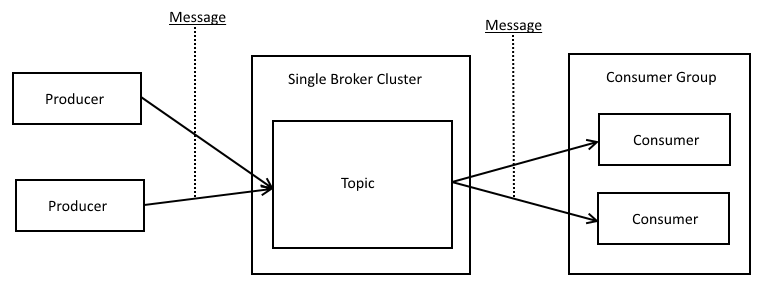
\includegraphics[width=1.0\textwidth]{bilder/kafkaDesign.png}
\caption{Apache Kafka Architektur - Single Broker Cluster
\label{fig:kafkaDesign}}
\end{figure}

%\citeint{kafka:documentation}

\begin{table}[ht!]
	\centering
		\begin{tabular}{@{}ll@{}} \toprule
			\textbf{Kriterium} & \textbf{Bewertung} \\ \midrule
			Architektur & Strukturierte Peer-to-Peer-Architektur \\
			Prozesse und Threads & Client-Server Cluster, Consumer Pull-Modell \\
			Kommunikation & TCP-basiert mit Apache Zookeeper \\
			Namenssystem & Hierarchische Benennung \\
			Synchronisierung & Consumer Groups, Stateless Broker \\
			Pipelining und Materialisierung & Publishing als Consumer \\
			Konsistenz und Replikation & Replikation \\
			Fehlertoleranz & Fail-Fast Strategie unter Supervision \\ %CRC removal of bad CRCs -> self healing?
			Sicherheit & Nur eigene Maßnahmen \\
			Erweiterung & Eigenentwicklung und Community-Beiträge \\
			Qualität & At-least-once delivery,  time-based SLA 7 Tage \\
			\bottomrule			
		\end{tabular}
	\caption{Bewertung Apache Kafka}
	\label{tab:bewkafka}
\end{table}